\documentclass[twocolumn, 11pt]{article}%
\usepackage{amsmath, amssymb, esint}
\usepackage{graphicx, cuted, geometry, float, chemfig}

\geometry{
    a4paper,
    total={170mm,260mm},
}

\begin{document}

\begin{strip}
  \vspace*{\dimexpr-\stripsep}
  \begin{center}
      \Large\textbf{FISIKA 2}\\
      \large{Pertemuan 2 - Minggu 1 (186405)}\\
      \large{\today}
   \end{center}
\end{strip}

\section{Lanjutan Hukum Coulomb}
        \paragraph{ } Karena, $ \displaystyle \hat r = \frac{\vec r}{\mid r \mid} $. Maka, hukum coulomb dengan notasi vektor adalah

        \begin{equation*}
            \begin{split}
                \vec F_{21} &= k \frac{q_1 . q_2}{r_{21}^2} \hat r_{21}\\\\
                \vec F_{21} &= k \frac{q_1 . q_2}{r_{21}^3} \vec r_{21}
            \end{split}
        \end{equation*}

        \subsection{Contoh}
        \paragraph{ } Kita ketahui bahwa $ \displaystyle \vec F_{12} = k \frac{q_1 . q_2}{r_{21}^2} \hat r_{21} $ dan

        \begin{equation*}
            \begin{split}
                \hat r_{12} &= \frac{\vec r_1 - \vec r_2}{r_{12}}\\
                &=\frac{(x_1 - x_2)\hat i + (y_1 - y_2)\hat j + (z_1 - z_2)\hat k}{\sqrt{(x_1 - x_2)^2 + (y_1 - y_2)^2 + (z_1 - z_2)^2}}\\
            \end{split}
        \end{equation*}

        Maka 
        \begin{equation*}
                \vec F_{12}\\
                = k q_1.q_2 \frac{(x_1 - x_2)\hat i + (y_1 - y_2)\hat j + (z_1 - z_2)\hat k}{((x_1 - x_2)^2 + (y_1 - y_2)^2 + (z_1 - z_2)^2)^{3/2}}\\
        \end{equation*}

        Untuk keterangan selanjutnya lihat \textbf{buku Fisika 2 Halaman 4, Contoh 1.1 dan Contoh 1.2}


\section{Medan Listrik dan Hukum Gauss}
    \subsection{Medan Listrik}
        \paragraph{ } Medan Listrik merupakan efek yang ditimbulkan oleh keberadaan ketidakseimbangan muatan listrik.
        \begin{center}
            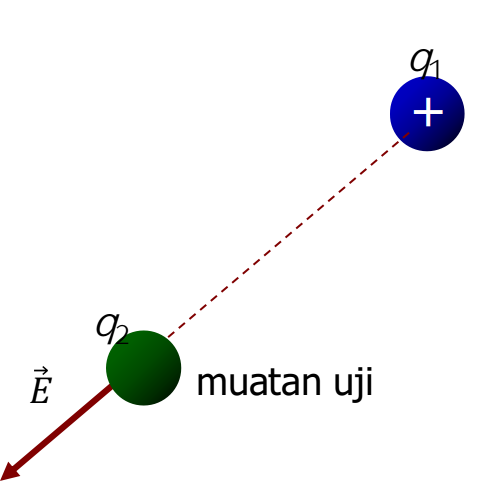
\includegraphics[width=100px]{0.png}
        \end{center}

        Muatan $q_1$ dapat melakukan gaya pada muatan $q_2$ meski kedua muatan tersebut tidak bersentuhan, karena adanya medan listrik. Jika besarnya medan listrik yang dihasilkan muatan $q_1$ pada posisi muatan $q_2$ dinyatakan dengan $\vec E_{21}$, maka gaya $q_2$ oleh $q_1$ adalah
        \[\vec F_{21} = q_2 \vec E_{21} \]\\
        
        Pada awal 1830-an, Faraday mengembangkan ide tentang medan listrik sebagai berikut:
        \begin{itemize}
            \item Sebuah partikel bermuatan menghasilkan “medan” ke segala arah dalam ruang.
            \item Partikel bermuatan yang lain merasakan medan tersebut, dan mampu “mengetahui” keberadaan muatan pertama
        \end{itemize}

        Arah medan listrik didefinisikan sebagai berikut:
        \begin{itemize}
            \item Arah medan listrik keluar dari Muatan (+) dan arah medan listrik masuk ke muatan (-)\\
                \begin{center}
                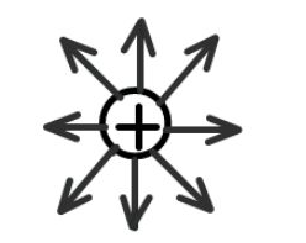
\includegraphics[width=80px]{1.png}
                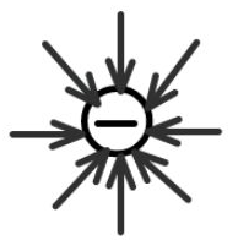
\includegraphics[width=80px]{2.png}
                \end{center}
        \end{itemize}
        
        Interaksi dua partikel bermuatan digambarkan sebagai berikut
        \begin{center}
            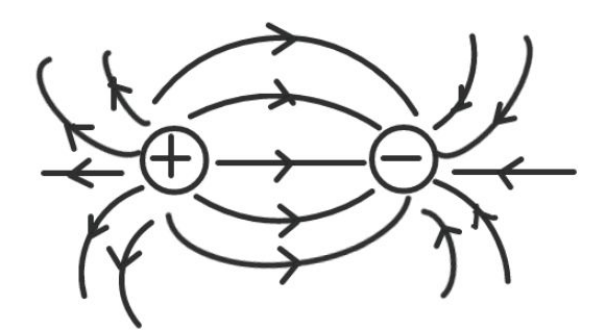
\includegraphics[width=100px]{3.png}
            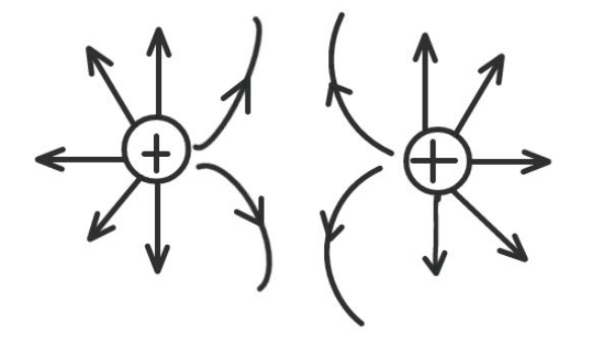
\includegraphics[width=100px]{4.png}
        \end{center}

        Sebagaimana gaya listrik, \textbf{medan listrik juga merupakan besaran vektor}. Jika ada gaya listrik yang bekerja pada suatu objek yang memiliki muatan $q_0$, maka medan listrik pada titik tersebut adalah:

        \begin{equation*}
            \begin{split}
            \vec E &= \frac{\vec F}{q_0}\\\\
            \vec E &= k \frac{q}{r^2} \hat r = k \frac{q}{r^3} \vec r
            \end{split}
        \end{equation*}
        
        N/C (tanda dari $q_0$ diikutsertakan). Mudahnya seperti ini, $q_0$ adalah muatan yang terkena medan. Sedangkan, $q$ adalah muatan yang mengeluarkan medan (yang mempengaruhi $q_0$).
        Jika bertanya-tanya kenapa penyebut $r^2$ bisa menjadi $r^3$, hal ini dikarenakan

        \[ \hat r = \frac{\vec r}{\mid r \mid} \]

        Medan listrik juga bisa dituliskan dengan formula/notasi kalkulus
        \[ \vec E = \lim_{\Delta q \to 0} \frac{\Delta \vec F}{\Delta q'} = \frac{d \vec F}{dq'} \]

    \subsection{Medan Listrik Oleh Beberapa Muatan Diskret}
        Karena medan listrik adalah besaran vektor, maka jika ada beberapa objek bermuatan, medan listrik total pada suatu titik akibat muatan-muatan tersebut merupakan \textbf{jumlahan vektor dari medan listrik setiap muatan}

        \begin{equation*}
            \begin{split}
                \vec E &= \sum_i \vec E_i\\
                &= \sum^n_{i=1} k \frac{q_i}{r_i^2} \hat r_i\\
                &= \sum^n_{i=1} k \frac{q_i}{r_i^3} \vec r_i
            \end{split}
        \end{equation*}

    \subsection{Gerakan sebuah partikel bermuatan di dalam medan listrik seragam}
        Partikel bermuatan di dalam medan listrik merasakan suatu gaya listrik, dan jika muatan ini bebas bergerak, maka percepatan gerak partikel dapat ditentukan.

        Jika satu-satunya penyebab gaya adalah medan listrik, maka

        \[\sum \vec F = m \vec a = q \vec E \]

        \begin{center}
        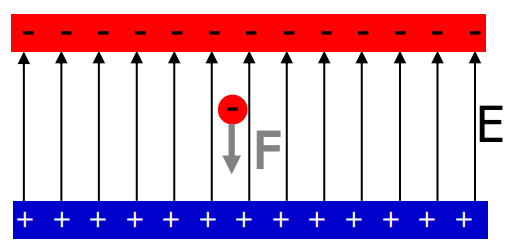
\includegraphics[width=150px]{5.png}
        \end{center}

        Jika $\vec E$ konstan, maka $\vec a$ juga konstan. Konsep kinematika gerak lurus (GLB, GLBB, Gerak parabola) dapat digunakan untuk menganalisa gerak muatan tersebut.

        Jika partikel bermuatan tersebut mempunyai $V_0$ yang tegak lurus arah medan listrik seragam, maka lintasan partikel tersebut akan berubah menjadi gerak parabola (mirip dengan melempar benda jatuh)

        \begin{center}
            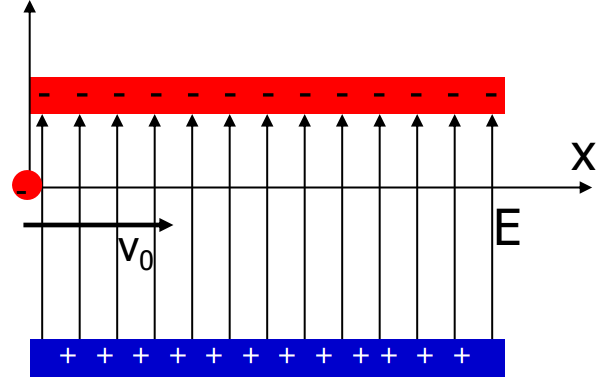
\includegraphics[width=150px]{6.png}
        \end{center}

        Aplikasi dari prinsip ini adalah pada \textbf{tabung sinar katoda} yang ada pada TV tabung atau Monitor komputer tabung. \textbf{Contoh penurunan rumus ada pada buku Fisika 2 halaman 6, contoh 1.3}.
        
        \begin{center}
            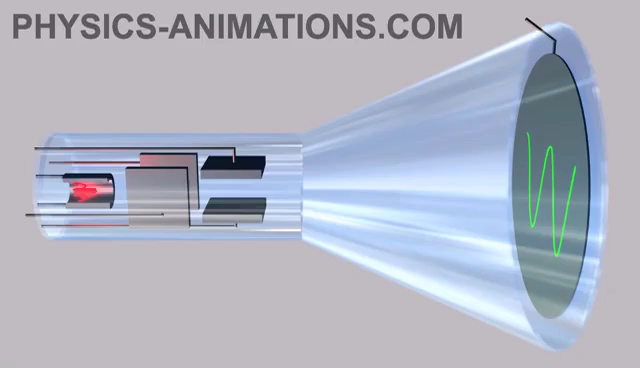
\includegraphics[width=150px]{7.png}
        \end{center}

        The cathode-ray tube, which is used to obtain a visual display of electronic information in oscilloscopes, radar systems, television receivers, computer monitors, etc.

\end{document}
